\xchapter{Publicização de software acadêmico de análise estática}
{Este capítulo apresenta um estudo sobre a publicização de 
de software acadêmico de análise estática divulgados nas conferências de
Engenharia de Software ASE e SCAM até o ano de 2015.}
\label{estudo1}

Este estudo selecionou, através de uma revisão de literatura em conferências da
Engenharia de Software, 60 projetos de software de análise estática
desenvolvidos e publicados nas conferências ASE e SCAM, caracterizou estes
projetos em relação a sua publicização, em termos de disponibilidade para download, acesso ao código fonte, forma de distribuição e licença.

A seção \ref{estudo1:introducao} contextualiza o estudo,
a seção \ref{estudo1:fundamentacao} apresenta os conceitos teóricos necessários para compreensão do trabalho,
a seção \ref{estudo1:definicao} descreve o objetivo e apresenta as questões de pesquisa,
a seção \ref{estudo1:planejamento} apresenta um planejamento do estudo,
as seções \ref{estudo1:preparacao} e \ref{estudo1:coleta} apresentam detalhes sobre a preparação e execução da coleta de dados,
as seções \ref{estudo1:analise} e \ref{estudo1:interpretacao} apresentam a análise e interpretação dos dados e
a seção \ref{estudo1:conclusoes} traça as conclusões finais deste estudo.

\section{Introdução e Motivação} \label{estudo1:introducao} % {{{

Os projetos de software desenvolvidos na academia sofrem de {\it
``dysfunctional chaotic churn''} \cite{howison2015understanding}.

Na prática, isso significa que há muitos projetos com características e
funcionalidades parecidas, com poucos usuários, com ciclos de vida curtos, e
encerrados quando o financiamento inicial termina, bem como, comunidades
desconectadas e paralelas, incompatibilidades entre projetos em um mesmo
domínio, e tentativas aparentemente não coordenadas de ``reiniciar'' tudo ({\it
re-boots}).

Parte deste problema tem sido atribuido a falta de treinamento em boas práticas
de desenvolvimento de software por parte dos cientistas e pesquisadores
\cite{wilson2017good}. Algo que, a princípio, não afeta os cientistas da
Engenharia de Software, visto que estes possuem formação e acesso a práticas de
desenvolvimento e estão inseridos num contexto voltado para a compreensão e
melhoria dos processos de desenvolvimento de software, tanto do ponto de vista
teórico, quanto prático.

Sabendo disso, e atentando para o fato que a grande parte do desenvolvimento de
software acadêmico é realizado pelos próprios cientistas \cite{hettrick2014uk,
momcheva2015software}, surge a preocupação de avaliar o quanto os projetos de
software desenvolvidos nas pesquisas de Engenharia de Software sofrem desse
problema, percebido por \citeonline{howison2015understanding} como
``dysfunctional chaotic churn''.

% }}}

\section{Fundamentação} \label{estudo1:fundamentacao} % {{{

\subsection{Software acadêmico}

São projetos de software desenvolvidos durante pesquisas científicas publicados
na literatura acadêmica, normalmente utilizados para coleta ou análise de
dados, podendo ser feito com objetivo de ser utilizado por outros
pesquisadores, e em algumas ocasiões sendo o software uma contribuição primária
para a Ciência \cite{howison2011scientific}.

\subsection{Disponibilidade/Publicização}

%Publicize your academic software
%Divulgação; ação de fazer com algo se torne público; realizar publicidade.

Disponibilidade neste estudo está relacionada a URL do projeto de software,
indicando se o software está disponível na URL indicada pelos seus autores e de
que forma os projetos estão disponíveis, binários ou código fonte, quais
licenças são utilizadas, entre outras questões relacionadas à distribuição.

% }}}

\section{Escopo} \label{estudo1:definicao} % {{{

Quantos projetos de software acadêmico de análise estática publicados
nas conferências ASE e SCAM permanecem disponíveis
hoje? Quais as informações que estão disponíveis?

\subsection{Definição do Objetivo}

\begin{description}
  \item{\bf Objeto de estudo.}
     O objeto de estudo são projetos de software acadêmico de análise estática.
  \item{\bf Propósito.}
    O propósito é caracterizar.
  \item{\bf Perspectiva.}
    A perspectiva considerada é a do cientista usuário final.
  \item{\bf Foco de qualidade.}
    O principal aspecto de qualidade estudado é a disponibilidade dos projetos.
  \item{\bf Contexto.}
    O estudo foi conduzido com publicações das conferências de Engenharia de Software ASE e SCAM.
\end{description}

\subsection{Sumário da Definição}

Analisar os \textit{projetos de software acadêmico de análise estática}
com o propósito de \textit{caracterizar}
com respeito a \textit{disponibilidade}
na perspectiva de \textit{cientistas usuários finais}
no contexto de \textit{conferências de Engenharia de Software ASE e SCAM}.

\subsection{Questões de Pesquisa}

Neste estudo as seguintes questões de pesquisa, a respeito dos projetos de
software acadêmico de análise estática publicados nas conferências ASE e SCAM,
serão investigadas:

\newcommand{\EstudoUmQuestaoUm}{
  Os projetos de software acadêmico de análise estática publicados nas conferências ASE e SCAM possuem alguma presença oficial online?
  %requisito para avaliar qualidade interna dos projetos
}
\newcommand{\EstudoUmQuestaoDois}{
  Os projetos de software academico de análise estática publicados nas conferências ASE e SCAM estão disponíveis para download?
  %requisito para uso
}
\newcommand{\EstudoUmQuestaoTres}{
  É possível ter acesso ao código fonte dos projetos de software de análise estática publicados nas conferências ASE e SCAM?
  %requisito para avaliar qualidade interna dos projetos
}
\newcommand{\EstudoUmQuestaoQuatro}{
  Os projetos de software com código fonte disponível podem ser adaptados para atender necessidades emergentes?
  %requisito para usar em novas pesquisas
}

\begin{description}
  \item [Q1:] \EstudoUmQuestaoUm
  \item [Q2:] \EstudoUmQuestaoDois
  \item [Q3:] \EstudoUmQuestaoTres
  \item [Q4:] \EstudoUmQuestaoQuatro
\end{description}

\subsection{Métricas}

Para responder às questões de pesquisas, as seguintes métricas serão usadas:

\begin{enumerate}
  \item Número de projetos com identificação de nome e URL
  \item Número de projetos com URL disponível
  \item Número de projetos disponíveis para download
  \item Número de projetos com código fonte disponível
  \item Número de projetos com permissão explícita de contribuição via código fonte
\end{enumerate}

% }}}

\section{Planejamento do Estudo} \label{estudo1:planejamento} % {{{

Este estudo foi realizado em duas etapas principais, conforme ilustrado na
Figura \ref{estudo1-etapas}. Na primeira etapa, uma revisão da literatura
foi realizada, com o objetivo selecionar
artigos com publicação de software acadêmico de análise estática. 
Na segunda etapa, os projetos de software selecionados foram caracterizados
em relação a disponibilidade de código.

\begin{figure}[h]
  \center
  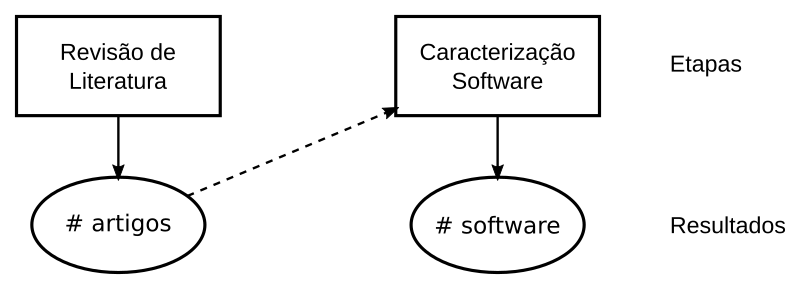
\includegraphics[scale=0.4]{imagens/estudo1-etapas.png}
  \caption{Etapas do estudo e seus resultados}
  \label{estudo1-etapas}
\end{figure}

%As seções a seguir apresentam o planejamento dessas duas etapas.

\subsection{Revisão de literatura com publicação de software de análise estática}

%Nesta primeira etapa realizamos um
O objetivo da revisão de literatura realizada foi %com o objetivo de
encontrar artigos mencionando software de análise estática entre os resultados
do estudo. A revisão foi organizada em três passos, detalhados a seguir.

%-- busca, filtro e seleção -- cada etapa 
%um conjunto de artigos que atendem aos critérios de inclusão e
%exclusão definidos naquela atividade, estes artigos são utilizados como entrada
%na etapa seguinte.  A última atividade -- seleção -- gera como saída o conjunto
%final de artigos com publicação de software acadêmico de análise estática.

\subsubsection{Passo 1: Escopo}

%de Engenharia de Software utilizadas como ponto de partida na revisão de literatura,

Este passo teve como objetivo a seleção das conferências a serem utilizadas como fonte dos
artigos para a revisão de literatura. 
Para cada conferência, todas as publicações serão selecionadas e
incluídas no conjunto inicial de artigos da revisão, iniciando pela primeira
edição de cada conferência indo até a última edição disponível no ano da execução da revisão.
%Assim, foram consideradas todas as publicações de cada conferência até o ano limite,
%incluindo os artigos publicados nesse ano.

As conferências devem ser selecionadas tendo em vista aumentar e potencializar
o número total de projetos de software acadêmico do domínio de aplicação de
interesse do estudo, neste caso, análise estática. Deve-se buscar
preferencialmente conferências com bom histórico de publicações sobre o domínio
de aplicação do estudo.

É importante investigar o histórico de cada conferência com atenção ao nome do
evento em cada edição, não é raro que conferências com muitos anos de
existência mudem de nome ao longo do tempo, nestes casos deve-se adotar o nome
da conferência mais recente e consider todas as edições anteriores com este
mesmo nome.

%, ou
%seja, o nome mais recente, mesmo que isto inclua conferencias distintas, é
%adotado para todas as edições.

Uma vez definidos a data limite e as conferências deve-se fazer o download de
todos os artigos até a data limite, os arquivos devem ser organizados em pastas
por nome e ano da conferência. Os títulos de todos os artigo, a correspondente
conferência e o ano de publicação devem ser registrados e armazenados em
arquivos ou banco de dados, neste estudo fizemos uso do
LibreOffice Calc\footnote{\url{https://www.libreoffice.org}}.

%O formato desta planilha , sobre a estrutura de pastas utilizadas
%para armazenar os artigos, e onde encontrar o arquivo utilizado neste estudo
%para a coleta destes dados pode ser consultado em detalhes no Apêndice
%\ref{reproducibilidade-do-estudo}.

\subsubsection{Passo 2: Triagem Automática} \label{estudo1:planejamento:filtro}

O escopo definido no passo anterior irá, potencialmente, resultar num enorme
conjunto de artigos para revisão. Assim, o objetivo da triagem automática é reduzir o tamanho deste
conjunto, mantendo apenas as publicações relevantes para os objetivos do estudo.

A triagem é realizada por meio de uma busca textual no conteúdo de cada artigo. A
busca deve ser realizada de forma automática com auxilio de ferramentas de
software para busca textual em conteúdo de arquivos pdf, com base em um %. Ela irá pesquisar um
conjunto de palavras-chave representando os critérios de inclusão da triagem.
Apenas os artigos combinando com estes critérios serão incluídos, conforme
Tabela \ref{criterios-triagem}.

\begin{table}[h]
\caption{Critérios de inclusão e palavras chave para a triagem dos artigos.}
\centering
\begin{tabular}{ l l }
  \hline
  Critério                                 & Palavras chave                        \\
  \hline
  Menciona projeto, software ou ferramenta & {\tt tool} ou {\tt framework}         \\
  Disponibiliza download do projeto        & {\tt download} ou {\tt available}     \\
  Identifica URL do projeto                & {\tt http} ou {\tt ftp}               \\
  Domínio de análise estática              & {\tt static analysis} ou {\tt parser} \\
  \hline
\end{tabular}
\label{criterios-triagem}
\end{table}

Se um determinado artigo não combinar com algum dos critérios ele será
excluído. Ao final da triagem, espera-se obter um conjunto reduzido
de artigos, contendo apenas as publicações relevantes para o objetivo
deste estudo.

%contendo apenas artigos com ocorrencia das palavras chave
%relacionadas a cada um dos critérios, este conjunto reduzido é passado para a
%etapa seguinte.

\subsubsection{Passo 3: Extração}

Os artigos incluídos serão inspecionados manualmente em busca de software acadêmico de
análise estática entre os resultados do estudo. Os critérios de inclusão têm
como objetivo incluir apenas os projetos de software identificados minimamente
pelos seus autores com nome e URL para download, conforme Tabela
\ref{criterios-extracao}.

\begin{table}[h]
\caption{Critérios de inclusão para o passo de extração dos artigos (adaptado de \citeonline{howison2016software}).}
\centering
\begin{tabular}{ l p{12cm} }
  \hline
  Critério         & Explicação \\
  \hline
  Identificável    & É possível identificar um projeto de software entre as contribuições do artigo? (ex: ``um programa que nós escrevemos``, ``nossa implementação``, ``nosso protótipo'') \\
  Disponível       & Podemos encontrar menção a URL do projeto de software para download? \\
  \hline
\end{tabular}
\label{criterios-extracao}
\end{table}

O nome e o endereço URL de cada projeto encontrado durante a inspeção manual
devem ser extraídos e armazenados junto aos dados já coletados nos passos
anteriores da revisão. A inspeção deve incluir a leitura do título, introdução,
resultados e conclusões de cada artigo e, caso necessário, outras
seções do artigo. Alguns artigos podem descrever a contribuição de software acadêmico
em seções específicas, por exemplo, em
notas de rodapé com a URL do software.

Os artigos devem ser inspecionados num ciclo, um por vez, até chegar ao útlimo
artigo dentre os selecionados no passo anterior. Ao final da extração, teremos
dados de um conjunto de projetos de software acadêmico de análise estática,
incluindo nome do projeto e URL para download. Estes dados extraídos devem ser
atualizados nos arquivos ou banco de dados já utilizados nos passos anteriores.

%A planilha LibreOffice Calc utilizada como apoio
%na revisão foi atualizada com o nome do software publicado no artigo
%correspondente.
%de artigos com publicação de

%Os critérios de seleção da Tabela \ref{criterios-selecao} foram adaptados do
%trabalho de \citeonline{howison2016software}, que fez uma revisão de literatura
%da Biologia em busca de menções a software acadêmico para evidenciar problemas
%de visibilidade e de uso.

\subsection{Caracterização dos projetos de software acadêmico de análise estática}

Os dados coletados na revisão de literatura, devidamente armazenados em
arquivos ou banco de dados, incluem projetos de software acadêmico de análise
estática, identificados com nome e URL, nome e ano da conferência e
título do artigo onde foi publicado.

Estes dados deverão ser extraídos para uma nova estrutura de armazenamento
projetada para receber informações adicionais dos projetos, conforme Tabela
\ref{esquema-caracteristicas}, essas informações serão coletadas em documentos
relacionados aos projetos, como website, manuais, repositórios e código fonte.

\begin{table}[h]
\caption{Esquema para caracterização dos projetos de software acadêmico}
\centering
\begin{tabular}{ l p{11cm} }
  \hline
  Característica           & Explicação \\
  \hline
  Nome do software         & O nome do projeto de software \\
  URL                      & Endereço web do software ou projeto, site ou repositório de código fonte, com o software disponível \\
  Título do artigo         & Título do artigo onde o software é citado como contribuição, seja principal ou secundária \\
  Nome do evento           & Nome da conferência onde o software foi publicado \\
  Ano do evento            & Ano da edição da conferência onde o artigo foi publicado \\
  Descrição do software    & A descrição do projeto de software \\
  Acesso                   & Podemos acessar a URL do projeto agora? Pode receber os seguintes valores: Sem Acesso, Acesso Pago, Acesso Gratuito \\
  Distribuição             & Como o software é distribuído e pode ser acessado? Pode receber os seguintes valores: gratis, livre, proprietário \\
  Código fonte disponível  & É possível acessar o código fonte de alguma forma? \\
  Licença                  & O software deixa explícito qual licença é distribuído? \\
  Código fonte             & Em qual linguagem de programação o software acadêmico foi desenvolvido \\
%  Entradas suportadas      & Qual o tipo de entrada suportada pelo software de análise estática \\
%  Linguagens suportadas    & Quais linguagens de programação o software de análise estática suporta como entrada \\
  \hline
\end{tabular}
\label{esquema-caracteristicas}
\end{table}

O primeiro documento consultado deve ser o website indicado pela URL, esta
consulta resultará em novos documentos, como, manuais de uso, informações sobre
desenvolvimento, código fonte, notas de lançamento, entre outros. Cada um
destes documentos devem ser inspecionados em busca de informações para
caracterização dos projetos segundo a Tabela \ref{esquema-caracteristicas}.

%e documentos para download no
%site, estes documentos, quando disponíveis, também foram consultados, estes
%documentos estão normalmente disponíveis em formato txt, pdf ou doc.
%Quando disponível, o código fonte também foi inspecionado em busca de
%informações, alguns projetos distribuem junto ao código fonte documentos e
%manuais, outros documentam informações sobre o projeto no próprio código.

A coleta sobre a linguagem de programação em que projeto está escrito deve ser
realizada de maneira automática através de alguma ferramenta de análise de
código fonte, como por exemplo o software livre
\texttt{sloccount}\footnote{http://www.dwheeler.com/sloccount}.

% }}}

\section{Preparação} \label{estudo1:preparacao} % {{{

Nesta seção apresentamos a preparação do estudo para a realização da coleta de
dados.

\subsection{Revisão de literatura com publicação de software de análise estática}

\subsubsection{Passo 1: Escopo}

Seguindo o planejamento descrito em \ref{estudo1:planejamento}, definimos como
fonte de busca as conferências SCAM\footnote{\url{http://www.ieee-scam.org}}
({\it Source Code Analysis and Manipulation Working Conference}) e
ASE\footnote{\url{http://ase-conferences.org}} ({\it Automated Software
Engineering}), ambas conferências com um grande histórico de edições, definimos
como data limite o ano de 2015.

Buscamos descobrir onde os artigos estão disponíveis para download, as
publicações da conferência SCAM estão todas disponibilizadas no IEEE, a
conferência ASE possui algumas edições no IEEE outras na ACM, os endereços URL
de cada edição de cada conferência estão documentadas no Apêndice
\ref{reproducibilidade-do-estudo}.

Até o ano de 1996 a conferencia ASE chamava-se KBSE - Knowledge-Based Software
Engineering Conference e a partir de 1997 passou a chamar-se ASE - Automated
Software Conference, teve sua primeira edição no ano de 1991 e o SCAM apenas em
2001.

\subsubsection{Passo 2: Triagem Automática}

%Definimos as palavras chave para a execução do filtro conforme planejado com
%o fim de selecionar apenas os artigos que casam com os critérios definidos
%na , estes critérios e as palavras chave
%associado à cada um são apresentados na Tabela \ref{criterios-filtro}.

%Estas palavras foram escolhidas de forma empírica e contam com experiência
%prévia na área de análise estática, notamos que usualmente os autores de
%software acadêmico de análise estática mencionam contribuição em software
%fazendo menção utilizando estes termos, de forma que consideramos que a
%aplicação deste filtro em outros domínios necessita de adaptações.

Implementamos o script para execução da triagem automática a partir dos
critérios definidos no planejamento, Seção \ref{estudo1:planejamento:filtro},
este script utiliza como base o software livre
\texttt{pdftotext}\footnote{\url{https://en.wikipedia.org/wiki/Pdftotext}} para
converter o conteúdo pdf dos arquivos em texto antes de realizar o filtro pelas
palavras chave.

\subsubsection{Passo 3: Extração}

Criamos uma planilha LibreOffice Calc para coletar os dados de cada passo da
revisão de literatura com as seguintes colunas:

\begin{description}
  \item[Evento] Nome e ano da conferência de Engenharia de Software.
  \item[Escopo] Título do artigo incluído no Passo 1: Escopo.
  \item[Triagem] 'SIM' se o artigo foi incluído no Passo 2: Triagem Automática.
  \item[Extração] 'SIM' se o artigo foi incluído na Passo 3: Extração.
  \item[Software] Nome do software identificado no artigo.
  \item[Anotações] Observações sobre o contexto em que o software é mencionado.
\end{description}

%que será utilizada durante 
%A única preparação necessária para esta atividade é se certificar que temos
%instalado um programa leitor de pdf para realização da inspeção manual dos
%artigos.

\subsection{Caracterização dos projetos de software acadêmico de análise estática}

Nesta fase de preparação para a caracterização dos projetos definimos a
estrutura de diretórios e nomes e formatos de arquivos utilizados para
armazenar os dados coletados, optamos por criar arquivos no formato YAML com o
nome \texttt{software.yml} para receber os dados do projeto e outro arquivo no
formato BibTeX chamado \texttt{paper.bib} para armazenar os dados do artigo
onde o software foi publicado.

%Definimos também o formato de armazenamendo das informações que serão
%coletadas
%optamos por utilizar arquivos no formato YAML organizados em
%diretórios por software, para cada software teremos um diretório contendo um
%arquivo chamado

Instalamos o software livre
\texttt{sloccount}\footnote{http://www.dwheeler.com/sloccount} para coletar a
linguagem de programação em que o projeto está escrito.

%acadêmico define-se quantos e quais são os projetos encontrados no conjunto de
%artigos selecionados na revisão de literatura, realizamos a verificação de
%quais são os projetos consultando a planilha LibreOffice Calc e para cada
%projeto criamos um diretório com o nome do software, o nome do software é antes
%transformado em minúsculas e removemos caracteres especiais, acentos, espaços
%em branco, este nome é utilizado para fazer referência ao software no restante
%do estudo.

% }}}

\section{Coleta de Dados} \label{estudo1:coleta} % {{{

Seguindo o planejamento e preparação descritos nas seções
\ref{estudo1:planejamento} e \ref{estudo1:preparacao} iniciamos a coleta dos
dados seguindo também duas grandes etapas, uma de revisão de literatura, outra
de caracterização dos projetos de software acadêmico.

\subsection{Revisão de literatura com publicação de software de análise estática}

A revisão de literatura encontrou 61 artigos com publicação de projeto de
software acadêmico de análise estática entre os 1873 artigos publicados nas
conferências ASE e SCAM, as atividades e resultados de cada passo da revisão
são representadas na Figura \ref{revisao-literatura}.

\begin{figure}[h]
  \center
  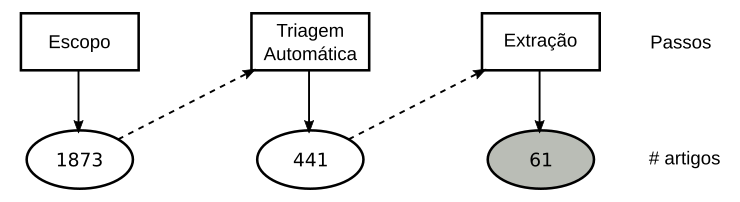
\includegraphics[scale=0.4]{imagens/revisao-literatura.png}
  \caption{Passos da revisão de literatura realizada nas conferências ASE e SCAM.}
  \label{revisao-literatura}
\end{figure}
% figura feita com base no artigo Nicolli Alves 2016, Fig 2

\subsubsection{Passo 1: Escopo}

A busca realizada nas conferências ASE e SCAM até o ano de 2015 resultou em
1873 artigos, deste total 346 artigos são do SCAM e 1527 artigos do ASE.

%Coletamos o título de cada artigo e armazenamos juntamente com o nome da
%conferência e edição onde o artigo foi publicado num arquivo do tipo ODS,
% detalhes sobre este
%arquivo pode ser encontrado no Apêndice \ref{reproducibilidade-do-estudo}.

\subsubsection{Passo 2: Triagem Automática}

O filtro executado automaticamente usando os critérios definidos na fase de
preparação reduziu o conjunto de 1873 para 441 artigos, 155 artigos do SCAM e
286 artigos do ASE, estes artigos serão inspecionados manualmente na atividade
seguinte.

\subsubsection{Passo 3: Extração}

Nesta atividade os 441 artigos foram inspecionados manualmente tendo como guia
os critérios descritos na Tabela \ref{criterios-extracao} na fase de
planejamento, selecionamos, nesta atividade, 61 artigos com publicação de
software acadêmico de análise estática

\subsection{Caracterização dos projetos de software acadêmico de análise estática}

Conforme planejado coletamos informações adicionais, descritas na Tabela
\ref{esquema-caracteristicas}, para cada projeto de software consultando
documentos de cada projeto, as informações coletadas são apresentadas, de forma
resumida, na Tabela \ref{software-table}.


\begin{longtable}{| l | l | l | l |}
\caption{Software acadêmico para análise estática.}
\label{software-table} \\
  \hhline{| l | l | l | l |}
  \hline
  \endfirsthead
  \hhline{| l | l | l | l |}
  \hline
  \textbf{Nome do software} & \textbf{Acesso} & \textbf{Código fonte} & \textbf{Distribuição} \\
  \hline
  \hhline{| l | l | l | l |}
  \endhead
  \hhline{|----|}
  \multicolumn{4}{|c|}{continua na próxima página} \\
  \hline
  \hhline{|----|} \endfoot
  \hhline{|----|} \endlastfoot
  \textbf{Nome do software} & \textbf{Acesso} & \textbf{Código fonte} & \textbf{Distribuição} \\
  \hline
    2LS &
      Gratuito &
      C++ &
      Livre \\
    AccessAnalysis &
      Gratuito &
      Java &
      Livre \\
    APIExample &
      Sem Acesso &
      - &
      - \\
    BEG &
      Sem Acesso &
      - &
      - \\
    ccJava &
      Sem Acesso &
      - &
      - \\
    CIVL &
      Gratuito &
      C &
      Livre \\
    CodeBoost &
      Gratuito &
      C &
      Livre \\
    CSL &
      Gratuito &
      C &
      Grátis \\
    CPA+ &
      Sem Acesso &
      - &
      - \\
    CSeq &
      Gratuito &
      C &
      Livre \\
    DDVerify &
      Sem Acesso &
      - &
      - \\
    Derailer &
      Gratuito &
      Ruby &
      Livre \\
    Diagnosys &
      Sem Acesso &
      - &
      - \\
    DOMPLETION &
      Gratuito &
      Javascript &
      Grátis \\
    DRC &
      Sem Acesso &
      - &
      - \\
    e-munity &
      Gratuito &
      C &
      Grátis \\
    EJB Interceptor Analyzer &
      Gratuito &
      Java &
      Grátis \\
    Error Prone &
      Gratuito &
      Java &
      Livre \\
    ESBMC &
      Sem Acesso &
      - &
      - \\
    ETXL &
      Sem Acesso &
      - &
      - \\
    FaultBuster &
      Gratuito &
      - &
      Grátis \\
    Flowgen &
      Gratuito &
      Python &
      Livre \\
    GRT &
      Sem Acesso &
      - &
      - \\
    GUIZMO &
      Gratuito &
      Java &
      Livre \\
    GumTree &
      Gratuito &
      Java &
      Livre \\
    HUSACCT &
      Gratuito &
      Java &
      Livre \\
    Indus &
      Gratuito &
      Java &
      Livre \\
    JastAdd &
      Gratuito &
      Java &
      Livre \\
    JFlow &
      Gratuito &
      Java &
      Livre \\
    JstereoCode &
      Sem Acesso &
      - &
      - \\
    Jtop &
      Sem Acesso &
      - &
      Livre \\
    Bogor/Kiasan &
      Gratuito &
      Java &
      Livre \\
    Loopfrog &
      Gratuito &
      - &
      Grátis \\
    Lotrack &
      Gratuito &
      Java &
      Grátis \\
    MPAnalyzer &
      Gratuito &
      Java &
      Grátis \\
    MSP &
      Sem Acesso &
      - &
      - \\
    mygcc &
      Gratuito &
      C &
      Livre \\
    PARSEWeb &
      Sem Acesso &
      - &
      - \\
    PAT &
      Sem Acesso &
      - &
      - \\
    PHP AiR &
      Gratuito &
      Rascal &
      Grátis \\
    protopurity &
      Gratuito &
      Javascript &
      Grátis \\
    Pseudogen &
      Gratuito &
      Python &
      Grátis \\
    PtYasm &
      Gratuito &
      Java &
      Grátis \\
    PuMoC &
      Sem Acesso &
      - &
      - \\
    PYTHIA &
      Sem Acesso &
      - &
      - \\
    ReAssert &
      Gratuito &
      Java &
      Livre \\
    Rêve &
      Sem Acesso &
      - &
      - \\
    RRFinder &
      Sem Acesso &
      - &
      - \\
    Sapid/XML &
      Sem Acesso &
      - &
      - \\
    Sonar Qube Plug-in &
      Gratuito &
      Java &
      Grátis \\
    SPARTA &
      Gratuito &
      Java &
      Grátis \\
    srcML &
      Gratuito &
      C++ &
      Livre \\
    SWAT &
      Sem Acesso &
      - &
      - \\
    TACLE &
      Gratuito &
      Java &
      Grátis \\
    TEBA &
      Gratuito &
      Perl &
      Grátis \\
    TestEra &
      Sem Acesso &
      - &
      - \\
    Vdiff &
      Sem Acesso &
      - &
      - \\
    WALA &
      Gratuito &
      Java &
      Livre \\
    Wrangler &
      Gratuito &
      Erlang &
      Livre \\
    XOgastan &
      Sem Acesso &
      - &
      - \\
  \hline
\end{longtable}



Dois artigos, entre os 61, fazem referência a um mesmo software, assim temos no
total 60 projetos de software selecionados, para cada projeto foi criado um
diretório contendo o nome do software e um arquivo chamado
\texttt{software.yml} com os dados coletados.

% }}}

% Raw results from the analysis
\section{Análise dos Dados} \label{estudo1:analise}

Coletamos 1873 artigos publicados nas conferências de Engenharia de Software
ASE e SCAM, selecionamos 61 artigos com publicação de software acadêmico de
análise estática, entre estes artigos caracterizamos 60 projetos de software,
coletamos para cada um ao menos nome e URL do projeto, e para cada projeto
informaçoes adicionais foram coletadas em fontes documentais diversas à respeito
do projeto, à seguir apresentamos a análise destes dados.

\subsection{Revisão de literatura com publicação de software de análise estática}

\subsubsection{Passo 1: Escopo}

A conferência ASE publica quase 4 vezes mais do que a conferência SCAM, a
edição com o maior número de publicações foi 2011 com 112 artigos publicados,
seguido de 2014 com 104, e 2007 com 102, a edição com o menor número foi 1996
com apenas 15 artigos publicados, A Figura \ref{artigos-por-ano} apresenta este
total distribuídos ao longo de cada edição.

\begin{figure}[h]
  \center
  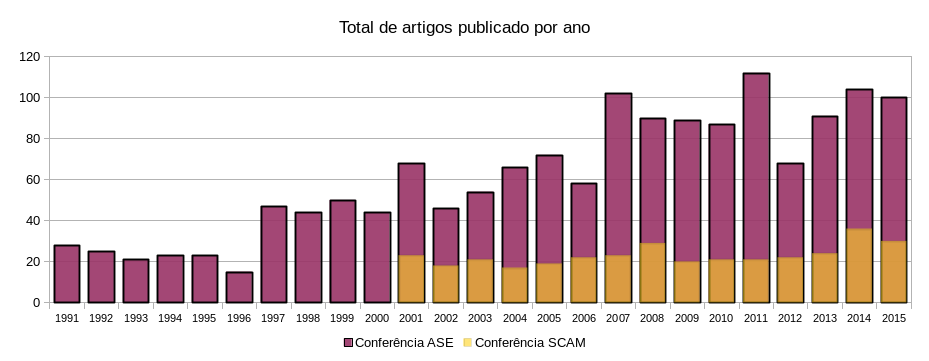
\includegraphics[scale=0.65]{imagens/artigos-por-ano.png}
  \caption{Total de artigos por ano publicados nas conferências ASE e SCAM.}
  \label{artigos-por-ano}
\end{figure}


\subsubsection{Passo 2: Triagem Automática}

Para a conferência ASE até o ano de 1996 nenhum artigo foi encontrado com
ocorrência das palavras chave utilizadas no filtro, apenas a partir de 1997
temos ocorrência dos termos pesquisados nas publicações desta conferência.

\subsubsection{Passo 3: Extração}

Considerando todo o período incluído na revisão de literatura encontramos uma
média de 2 artigos por ano com publicação de software acadêmico, a Figura
\ref{artigos-com-software-por-ano} apresenta os resultados distribuídos por
ano.

\begin{figure}[h]
  \center
  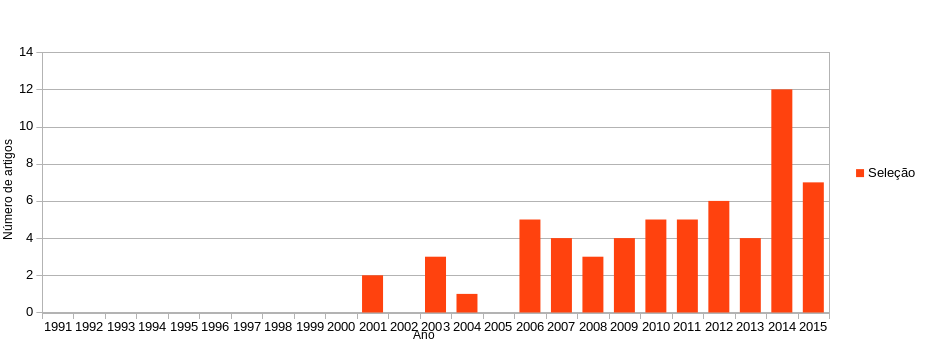
\includegraphics[scale=0.65]{imagens/artigos-com-software-por-ano.png}
  \caption{Artigos com publicação de software acadêmico selecionados na revisão de literatura.}
  \label{artigos-com-software-por-ano}
\end{figure}

A revisão de literatura teve como critério primordial encontrar publicação de
software com indicação de URL para download, ainda assim, no processo de
revisão encontramos 51 projetos sem indicação de URL para download, 30 projetos
na conferência ASE e 21 projetos na conferência SCAM.

%Os 30 projetos sem indicação de URL encontrados no ASE são:
%AGENDA, Rostra, VisAXSM, Jink, AMNESIA, ISIS4J, Decor, Smack, CBFA, iMaus,
%CPPCHECKER, Tikanga, Doc2Spec, Drails, ClassSplitter, UMGAR, Secoria,
%Impendulo, BEST, DC2, WAIVE+, COPES, Ranger, ProgramCutter, Scoria, Relda,
%CONBOL, SymCrash, CodeHow, SAFEWApp.

%Os 21 projetos sem indicação de URL encontrados no SCAM são:
%ReWeb, DMS, EMBER, VADA, ADiMat, AMOEBA, JSysDG, MAGIC, SCATR, ELAN, HaRe,
%X-DEVELOP, SUDS, Goanna, Parfait, Templar, MemSafe, CAWDOR, LIBCROOS, GASR,
%PtrTracker.

% Hypothesis rejection
\section{Interpretação dos Resultados} \label{estudo1:interpretacao}

\subsection{Q1 - \EstudoUmQuestaoUm} % presença online

Dos 60 projetos de software estudados neste trabalho, 15 não tem presença
oficial online no endereço de URL informado pelos seus autores, 45 projetos estão presentes através da
URL informada de alguma forma, significando que a URL informada pelos autores
estão ativas e online. %, alguns destes projetos ...

\subsection{Q2 - \EstudoUmQuestaoDois} % download

Entre os 60 projetos selecionados 24 não estão disponível para download, ou
seja, apesar dos autores informar no estudo uma URL, indicar que o software
está disponível nesta URL para download, a URL não mais está disponível e o
software não pode ser encontrado, ou seja, 40\% dos projetos de software
acadêmico de análise estática publicados nas conferências de Engenharia de
Software ASE e SCAM não estão disponíveis.

Os demais 36 projetos, que equivalem a 60\% do conjunto total, estão
disponíveis para download e é possível obter uma cópia destes projetos na URL
indicada pelos seus autores, um resumo deste total por ano é apresentado na
Tabela \ref{available-table}.



\begin{table}[h]
\caption{Número de projetos disponível para download por ano.}
\centering
\begin{tabular}{| l | c | c | c |}
  \hline
  {\bf Ano} & {\bf Total} & {\bf Disponível} & {\bf Indisponível} \\
  \hline
  2001 & 2 & 1 & 1 \\
  2003 & 3 & 1 & 2 \\
  2004 & 1 & 0 & 1 \\
  2006 & 5 & 4 & 1 \\
  2007 & 4 & 1 & 3 \\
  2008 & 2 & 1 & 1 \\
  2009 & 4 & 2 & 2 \\
  2010 & 5 & 3 & 2 \\
  2011 & 5 & 2 & 3 \\
  2012 & 6 & 2 & 4 \\
  2013 & 4 & 2 & 2 \\
  2014 & 12 & 11 & 1 \\
  2015 & 7 & 6 & 1 \\
  \hline
  {\bf Total} & 60 & 36 & 24 \\
  \hline
\end{tabular}
\label{available-table}
\end{table}



%Existe uma leve tendência, ao longo dos anos,  para a indisponibilidade das
%fontes informadas e páginas web.  É possível notar que, em 2006, 80\% de todos
%os softwares de análise estática publicados nas conferências ASE e SCAM ainda
%estão disponíveis.  Este número cresce em 2014, chegando a 90\%, e cai no ano
%seguinte para 85\%.  Apesar de não estar sempre crescente, e da  amostra
%pequena usada neste estudo -- apenas 60 projetos de software acadêmico, este
%leve indício confirma a afirmação de \citeonline{robles2010replicating}.

\subsection{Q3 - \EstudoUmQuestaoTres} % codigo fonte

Do conjunto de 36 projetos de software disponível para download, apenas 2 não
disponibilizam o código fonte, estão disponíveis apenas em formato binário, são
FaultBuster e Loopfrog, ambos disponibilizados gratuitamente mas apenas em
formato binário. A Tabela \ref{source-code-table} traz um resumo de quais
linguagens de programação estes softwares são escritos.

%Do conjunto de 60 projetos de software estudados, %% Joenio, coloquei aqui o tempo no PRETERITO -- revisar outras partes.
%3 não disponibilizaram seu código fonte e  %% Joenio, mudei as frases para VOZ ativa, sujeito: projeto de software.
%34 disponibilizaram o código fonte publicamente.



\begin{table}[h]
\caption{Linguagem de programação dos projetos com código fonte disponível.}
\centering
\begin{tabular}{| l | c |}
  \hline
  {\bf Linguagem de programação} & {\bf Número de projetos} \\
  \hline
  C & 6 \\
  C++ & 2 \\
  Erlang & 1 \\
  Java & 18 \\
  Javascript & 2 \\
  Perl & 1 \\
  Python & 2 \\
  Rascal & 1 \\
  Ruby & 1 \\
  \hline
\end{tabular}
\label{source-code-table}
\end{table}



\subsection{Q4 - \EstudoUmQuestaoQuatro} % licença

Dentre os 34 projetos que disponibilizaram o código fonte, 13 não informaram
licença alguma e 19 informaram licenças de FOSS ({\it free and open source
software}), a Tabela \ref{license-table} resume as licenças utilizadas e o
número de projetos em cada uma.



\begin{table}[h]
\caption{Licenças de software dos projetos com código fonte disponível.}
\centering
\begin{tabular}{| l | c |}
  \hline
  {\bf Licença de software} & {\bf Número de projetos} \\
  \hline
  Affero General Public License & 1 \\
  Apache License & 2 \\
  BSD License & 4 \\
  Eclipse Public License & 3 \\
  FrontEndART Software Ltd & 1 \\
  GNU General Public License & 6 \\
  GNU Lesser General Public License & 1 \\
  Illinois/NCSA Open Source License & 2 \\
  SAnToS Laboratory Open Academic License & 1 \\
  (sem licença) & 13 \\
  \hline
\end{tabular}
\label{license-table}
\end{table}



Todo software com o código fonte disponível pode ser adaptado para uso pessoal
sem qualquer restrição prévia pelos seus autores, mas os 13 projetos sem
licença definida impedem eventuais cientistas a publicar suas modificações e
redistribuir qualquer melhoria sem prévia solicitação aos autores originais.

Considerando o total de 60 projetos selecionados neste estudo, apenas 32\% (19
projetos) podem ser adaptados, os demais, 68\% (41 projetos) podem ser
adaptados mas as melhorias ou correções não podem ser redistribuídas sem
autorização prévia dos autores.

\section{Ameaças à validade}

O passo de triagem automática dos artigos no processo de revisão de literatura
pode ter excluído do processo de revisão algumas publicações com software
acadêmico de análise estática, fazendo o conjunto total de projetos
selecionados escapar algum projeto, apesar disso, o estudo tem como objetivo
caaracterizar os projetos e não as conferências em sí, de forma que esta ameaça
não causa impacto nas conclusões finais do estudo.

O escopo do estudo foi reduzido ao domínio de análise estática, portanto as
conclusões e interpretações estão limitadas neste contexto, acreditamos que
outros domínios de aplicação possui características semelhantes, mas é
conhecido que o domínio de aplicação é um fator de influência relevante nas
características dos produtos de software.

A leitura dos artigos na revisão, na fase final de Extração, foi realizado
apenas pelo autor deste trabalho, é certo que poderíamos aumentar a validade
realizando a revisão em par e revisados por outros pesquisadores.

O contexto selecionado com apenas duas conferências nos leva a possibilidade de
ter resultados com viés atrelado a estes dois eventos, é possível que as
características dos projetos publicados em outras conferências da Engenharia de
Software apresentem situação diferentes.

\section{Conclusões} \label{estudo1:conclusoes}

Este estudo selecionou 60 projetos de software de análise estática de código
fonte publicados nas conferências ASE e SCAM, todos identificados com nome do
projeto e URL para download. Os autores afirmam que os projetos estão
disponíveis para obtenção na URL indicada, mas os resultados da caracterização
feita mostram que apenas uma parcela destes projetos continuam disponíveis.

Entre os 60 projetos selecionados, 15 não têm qualquer presença oficial online,
com a URL indicada pelos autores indisponível. As únicas informações
disponíveis destes 15 projetos são aquelas encontradas nos artigos onde foram
publicados.

Nos 45 projetos com presença online através da URL informada nos artigos,
9 não disponibilizam qualquer artefato relacionado ao software, ou seja, apesar de ser
possível acessar a URL, não é possível encontrar o software para download.

Os 36 projetos restantes, com URL informada, estão disponíveis para download. A maior
parte dos projetos disponibiliza o código fonte na URL informada, sendo que 2 estão disponíveis
apenas em formato binário. Entre os projetos com código fonte disponível,
uma parcela deixa explícito qual licença e de que forma o software é
distribuído. ????

Dentre os 34 projetos com código fonte disponível, 13 não informam qualquer
licença de uso e, dessa forma, impedem que melhorias e correções
sejam distribuídas sem antes haver uma solicitação prévia aos autores destes
projetos. Finalmente, 19 projetos utilizam licenças de software livre e dão
prévia autorização para receber melhorias em código fonte.

É conhecido que os projetos de software desenvolvidos na academia não são ainda
reconhecidos pela Ciência como cidadãos de primeira classe, mesmo quando tais
projetos são indispensáveis para a compreensão dos estudos em que foram
desenvolvidos, neste estudo mostramos que uma grande parte (40\%) de um
conjunto de projetos de software acadêmico minimamente identificados pelos seus
autores com nome e URL encontram-se hoje indisponíveis.

No entanto, nao sabemos quais fatores influenciam um projeto estar ou não
disponível, e ainda, como tais projetos são vistos por outros pesquisadores, se
são utilizados e referenciados por outros autores, assim planejamos dois
estudos para investigar tais questões, apresentados nos próximos capítulos.

% Is sustainability a good predictor of citation rates for the software?
%"sustainability - turn out to be excellent predictors of citation rates for the software. Even the citations themselves will be different. "Another cool method also exists (Weasel et al. 2008)." versus "We used Weasel et al. (2008) to do amazing things" - which is a huge difference for us as programmers, I think! And when we are on hiring committees, we can very easily see how often your papers are getting cited."

%Percebemos também que existe uma grande quantidade de projetos de software
%publicados nestas duas sem indicação alguma de URL para obtenção do software,
%indicando que a ...

%detalhes sobre o formato YAML, estrutura utilizada para armazenamento e
%instalação estão documentados no Apêndice \ref{reproducibilidade-do-estudo}.

%Detalhes sobre o funcionamento do script de fitro, código fonte e instruções
%de uso podem ser consultados no Apêndice \ref{reproducibilidade-do-estudo}.

%Instruções de uso do sloccount e como ele foi utilizado neste estudo está
%documentado no Apêndice \ref{reproducibilidade-do-estudo}.

%com estas palavras num script, instalamos todas as suas
%dependências de execução, os detalhes de instalação e forma de uso deste script
%e suas dependências são documentados no Apêndice
%\ref{reproducibilidade-do-estudo}.

%% Planejamos fazer outro estudo ... 
